\chapter{Framework}\label{chapter:framework}
This chapter presents \gls{drispi}, the framework this thesis develops for the \gls{cvrp} at very-large scale (Section~\ref{sec:lit-problem}). \gls{drispi} repeatedly executes a decompose-route-improve (\gls{dri}) loop. Each iteration first partitions the customer set into smaller subclusters and solves one routing subproblem per subcluster with an existing monolithic solver. It then concatenates the resulting routes and revises them near the subcluster boundaries with a dedicated improvement stage, boundary-guided adaptive iterated local search (\gls{bg-ails}). Hierarchical adaptive operator selection (\gls{haos}) draws the decomposition and routing configuration for every iteration from a set of weighted alternatives and updates those weights from the outcomes it observes, rather than fixing one configuration for the whole run. Every route the \gls{dri} loop produces enters a persistent route pool. At scheduled intervals, \gls{drispi} then steps back from the current incumbent and recombines the pool through a set covering or set partitioning (\gls{sc}/\gls{sp}) model, followed by one further post-\gls{sc}/\gls{sp} improvement pass. The loop continues until a wall-clock time limit is reached.

Figure~\ref{fig:dri-overview} shows the resulting control flow for one instance. \gls{haos} (Section~\ref{sec:fra-haos}) draws one configuration per iteration. Decomposition (Section~\ref{sec:fra-decomposition}) partitions the customer set into $k$ subclusters under that configuration. The routing stage (Section~\ref{sec:fra-routing}) solves each subcluster independently and concatenates the routes. \gls{bg-ails} (Section~\ref{sec:fra-bg-ails}) revises the routes near the subcluster boundaries. Both the routing stage and \gls{bg-ails} add their routes to the route pool, and either can become the new incumbent if it improves on the current one. At scheduled intervals, the same iteration also runs set covering or set partitioning (Section~\ref{sec:fra-sp}) over the routes accumulated in the pool so far, followed by one further post-recombination improvement pass (Section~\ref{sec:fra-improve}) whose output feeds the pool again and can likewise become the new incumbent. If there is no \gls{sc}/\gls{sp} iteration scheduled, the loop either returns to a fresh \gls{haos} draw or stops. Figure~\ref{fig:dri-overview} shows this control flow as one sequential loop for illustrative purposes. Section~\ref{sec:fra-pipeline} then shows how \gls{drispi} executes it with several stages running in parallel across iterations instead.

The remaining sections address one stage each, in the order Figure~\ref{fig:dri-overview} shows: Section~\ref{sec:fra-haos} on \gls{haos}, Section~\ref{sec:fra-decomposition} on decomposition, Section~\ref{sec:fra-routing} on routing, Section~\ref{sec:fra-bg-ails} on \gls{bg-ails}, Section~\ref{sec:fra-sp} on the route pool and \gls{sc}/\gls{sp}, and Section~\ref{sec:fra-improve} on the post-\gls{sc}/\gls{sp} improvement pass. Section~\ref{sec:fra-pipeline} closes the chapter by assembling these stages into the parallelized pipeline \gls{drispi} actually runs, along with the pseudocode for its full loop.

\begin{figure}[H]
\centering
\begin{tikzpicture}[
  font=\small,
  >={Latex[length=2mm]},
  line/.style={draw, thick, ->},
  box/.style={rectangle, draw, thick, fill=black!4, align=center,
              minimum width=5.6cm, minimum height=0.9cm, inner sep=3pt},
  phase/.style={box, fill=blue!6},
  lane/.style={rectangle, draw, thick, fill=blue!6, align=center,
               minimum width=1.6cm, minimum height=0.8cm, inner sep=2pt},
  term/.style={ellipse, draw, thick, fill=black!10, minimum width=2.2cm, minimum height=0.8cm},
  dec/.style={diamond, draw, thick, fill=orange!8, align=center, aspect=3.2,
              inner sep=1pt, minimum width=5.6cm},
  tag/.style={rectangle, draw, thick, fill=blue!30!black!80, text=white,
              font=\small\bfseries\sffamily, minimum width=0.75cm, inner sep=0pt},
  bar/.style={fill=black, inner sep=0pt, minimum height=3pt},
  lbl/.style={font=\footnotesize},
]
\def\W{5.6cm}

\node[term]                          (start) {Start};
\node[box,   below=0.6cm of start]   (haos)  {\gls{haos} draws a configuration};
\node[phase, below=0.6cm of haos]    (dec)   {Decomposition into $k$ subclusters};

\node[bar, minimum width=4.8cm, below=0.55cm of dec] (fork) {};
\node[lane, below=0.4cm of fork]           (l2) {$\cdots$};
\node[lane, left=0.2cm of l2]              (l1) {Solve $\mathcal{P}_1$};
\node[lane, right=0.2cm of l2]             (l3) {Solve $\mathcal{P}_k$};
\node[bar, minimum width=4.8cm, below=0.4cm of l2] (join) {};
\node[draw, thick, dashed, rounded corners=2pt, inner xsep=0pt, inner ysep=5pt,
      minimum width=\W, fit=(fork)(join)(l1)(l3)] (route) {};

\node[phase, below=0.6cm of route]   (bg)    {\gls{bg-ails}};
\node[dec,   below=0.5cm of bg]      (q1)    {\gls{sc}/\gls{sp} scheduled?};
\node[phase, below=0.5cm of q1]      (sp)    {\gls{sc}/\gls{sp}};
\node[phase, below=0.6cm of sp]      (imp)   {Post-\gls{sc}/\gls{sp} Improvement};
\coordinate[below=0.5cm of imp]      (merge);
\node[dec,   below=0.5cm of merge]   (q2)    {Stopping criterion met?};
\node[term,  below=0.5cm of q2]      (end)   {End};

\foreach \n/\t in {dec/D, bg/I, sp/SP, imp/I}
  \node[tag, anchor=east, minimum height=0.9cm] at (\n.west) {\t};
\path let \p1=($(route.north)-(route.south)$) in
  node[tag, anchor=north east, minimum height=\y1] at (route.north west) {R};

\draw[line] (start) -- (haos);
\draw[line] (haos)  -- (dec);
\draw[line] (dec)   -- (fork);
\foreach \l in {l1,l2,l3} {
  \draw[line] (fork.south -| \l) -- (\l);
  \draw[line] (\l) -- (join.north -| \l);
}
\draw[line] (join) -- node[lbl, right, pos=0.45] {concatenate} (bg);
\draw[line] (bg)   -- (q1);
\draw[line] (q1)   -- node[lbl, right] {yes} (sp);
\draw[line] (sp)   -- (imp);
\draw[thick] (imp.south) -- (merge);
\draw[line] (merge) -- (q2);
\draw[line] (q2)   -- node[lbl, right] {yes} (end);

\def\xin{-4.0cm}
\def\xout{-4.9cm}
\draw[thick] (q1.west) -- node[lbl, above] {no} (\xin, 0 |- q1.west)
            |- (merge);
\fill (merge) circle (1.6pt);

\draw[line] (q2.west) -- node[lbl, above] {no} (\xout, 0 |- q2.west)
            |- node[lbl, pos=0.25, sloped, above] {next iteration} (haos.west);

\def\xpool{4.6cm}
\path let \p1=($(route.north)-(imp.south)$) in
  node[draw, thick, dashed, fill=black!3, minimum width=1.7cm,
       minimum height=\y1, anchor=north, align=center] (pool)
  at (\xpool, 0 |- route.north) {};
\node[align=center, font=\small] at (pool.center) {Route\\Pool};

\draw[line] (route.east) -- node[lbl, above] {feed} (pool.west |- route.east);
\draw[line] (bg.east)    -- node[lbl, above] {feed} (pool.west |- bg.east);
\draw[line] (pool.west |- sp.east) -- node[lbl, above] {read} (sp.east);
\draw[line] (imp.east)   -- node[lbl, above] {feed} (pool.west |- imp.east);
\end{tikzpicture}
\caption[Sequential Flowchart of DRISPI]{Sequential Flowchart of \gls{drispi}.}
\label{fig:dri-overview}
\end{figure}

\section{Hierarchical Adaptive Operator Selection}\label{sec:fra-haos}
Ideally, a heuristic would always be tuned to no more than one specific problem instance. That would promise both, an effective and efficient exploitation of that instance's structural characteristics such as size, spatial and demand distributions, or fleet capacity. Recent benchmark sets, however, have deliberately combined a wide range of these characteristics to test whether performance transfers across instance structures \citep{queirogaXLInstancesCapacitated2026,uchoaNewBenchmarkInstances2017}. That is why finding and selecting a tailored configuration for every instance requires a costly tuning campaign. Most benchmarks are therefore compromising on one fixed configuration for the entire problem set. This framework aims to forgo this compromise through Hierarchical Adaptive Operator Selection (\gls{haos}), an approach to adapt \gls{drispi}'s configuration while solving the problem instead.

The principal methodological inspiration is adaptive large neighborhood search, in which competing destroy and repair operators receive weights based on observed performance and are selected by roulette wheel \citep{ropkeAdaptiveLargeNeighborhood2006}. The same adaptive layer has been applied across five vehicle routing variants \citep{pisingerGeneralHeuristicVehicle2007}. \gls{haos} adopts this principle but moves the adaptive choice outside a single local search. It instead controls the decomposition granularity, the representation and method used for clustering, the demand contribution to cluster formation, as well as the subsolver. The adaptation is online because rewards update the weights while the current instance is being solved. The weights of each operator summarize observed performance on that instance. The convergence to a globally optimal configuration is neither required nor guaranteed.

The operator choices can also be interpreted as arms of a multi-armed bandit. After an arm is drawn, the search observes a reward but does not know what the unselected arms would have produced. This analogy connects \gls{haos} to the exploration--exploitation problem \citep{auerFinitetimeAnalysisMultiarmed2002} and to bandit-based adaptive operator selection \citep{fialhoAnalyzingBanditbasedAdaptive2010}. However, \gls{haos} does not implement a confidence-bound policy, an explicit exploration bonus, or a separate exploratory action. Its roulette probabilities follow the current weights directly. Stochastic sampling leaves every positive-weight option selectable, while a probability-floor transformation raises normalized shares that become sufficiently small.

At the beginning of every \gls{dri} iteration \gls{haos} draws one configuration across five levels:
\begin{itemize}
  \item Level one selects the number of subclusters $k$ from a scale-adaptive domain. Its base values are clipped to the instance's minimum feasible fleet size and extended geometrically for larger instances. The number of arms is capped at ten to allow for convergence to occur within a reasonable wallclock time.
  \item Level two selects the demand weight $\lambda_q$ from six evenly spaced values between zero and one. $\lambda_q$ controls how strongly differences in customer demand influence the decomposition.
  \item Level three selects the clustering paradigm $\pi$: whether customers are clustered directly (the vertex-based paradigm) or through the routes of the current incumbent solution (the route-based paradigm).
  \item Level four selects a clustering method $m$ from the wheel associated with $\pi$, with five vertex-based and three route-based clustering methods respectively. This conditional fourth level makes the selection hierarchical since the selection of $m$ depends on $\pi$.
  \item Level five selects one of four routing solvers $s$ and applies it to every subcluster generated during the iteration.
\end{itemize}
The first four levels therefore configure decomposition, and the fifth configures subproblem routing. A full five-level configuration is expressed as $\theta = (k, \lambda_q, \pi, m, s)$.

Two feasibility adjustments apply before the configuration is used. First, route-based clustering requires an incumbent solution. Without one, \gls{haos} uses the vertex-based paradigm and redraws the method from the vertex wheel. Second, if $k$ exceeds the number of incumbent routes under route-based clustering, the applied $k$ is clipped to the route count. Algorithm~\ref{alg:haos} shows the resulting functions $Draw$, $Credit$, and $Decay$. Each iteration is logged with the complete operator selection and the product of the five selected probabilities, which reports the joint probability of the realized configuration under the current wheels.

\begin{algorithm}[tbp]
\caption{Hierarchical Adaptive Operator Selection (\gls{haos})}\label{alg:haos}
\KwIn{wheels $W_1, W_2, W_3, W_4^{\mathrm{v}}, W_4^{\mathrm{r}}, W_5$; floors $p_{\min}^{(\ell)}$; decay $\gamma$; base weight $w_0$; warm-up $i_0 = 10$}
\BlankLine
\Fn{\Draw{$S^\star$}}{
  draw $k$, $\lambda_q$, $\pi$, $s$ from $W_1, W_2, W_3, W_5$ with probabilities (\ref{eq:haos-probability})\;
  \lIf{$\pi = \text{route}$ \KwAnd $S^\star$ is undefined}{$\pi \gets \text{vertex}$}
  draw method $m$ from $W_4^{\pi}$\;
  $\theta \gets (k, \lambda_q, \pi, m, s)$ \tcp*[r]{credited}
  \lIf{$\pi = \text{route}$}{$k \gets \min(k, |S^\star|)$}
  \Return credited $\theta$ and applied $(k, \lambda_q, \pi, m, s)$\;
}
\BlankLine
\Fn{\Credit{$\theta, r$}}{
  \lIf{$i \geq i_0$}{$w_a \gets \max(w_a + r,\, w_0)$ for every arm $a \in \theta$ by (\ref{eq:haos-update})}
}
\BlankLine
\Fn{\Decay{}}{
  \lIf{$i \geq i_0$}{$w_a \gets \max(\gamma w_a,\, w_0)$ for every arm of every wheel by (\ref{eq:haos-decay})}
}
\end{algorithm}

\gls{haos} maintains six roulette wheels for the five levels because of the conditional clustering method on the fourth level. Each wheel tracks one weight per option. A reward $r$ adds to the weight of every arm selected for the credited configuration. Once per iteration, every weight is also multiplied by a common decay factor. This uniform decay is the only temporal mechanism in the weights. Both operations retain the starting weight as a lower bound:
\begin{align}
w_i &\leftarrow \max(w_i + r,\ w_0), \label{eq:haos-update}\\
w_i &\leftarrow \max(\gamma w_i,\ w_0), \qquad \gamma = 0.95 \text{ by default,} \label{eq:haos-decay}
\end{align}
with every wheel starting from the same flat weight of $w_0~=~10.0$.  Before an arm is drawn, \gls{haos} first computes its normalized weight $\hat{p}_i = w_i / \sum_l w_l$. A level-specific floor is applied to these values, followed by renormalization:
\begin{equation}
p_i = \frac{\max(\hat{p}_i,\ p_{\mathrm{min}})}{\sum_j \max(\hat{p}_j,\ p_{\mathrm{min}})}.
\label{eq:haos-probability}
\end{equation}
The floor parameter is the minimum probability any weight of any wheel can decay to. For the five levels, the floors are 0.025 for $k$, 0.05 for $\lambda_q$, the clustering methods, and the solver, and 0.10 for the paradigm. Because Equation~\ref{eq:haos-probability} renormalizes after flooring, these values are nominal pre-normalization floors rather than strict lower bounds on the final probabilities. \gls{haos} retains three elements of the adaptive layer proposed by \citet{ropkeAdaptiveLargeNeighborhood2006} and used for general vehicle routing by \citet{pisingerGeneralHeuristicVehicle2007}: initially equal weights, quality-dependent scores, and roulette selection proportional to the resulting weights. Its additive reward, global decay, and six-wheel hierarchy are novelties introduced for \gls{drispi}\@.

\gls{haos} adapts its weights by receiving rewards from later stages of the current or following iterations. First, there is an immediate channel for results produced directly by the current \gls{dri} iteration and a deferred channel for routes that prove useful during later pool recombinations. Table~\ref{tab:haos-rewards} shows the deployed reward values. Both channels compare a candidate with the incumbent best cost and the previous iteration's cost, but the deferred scores are smaller because several earlier configurations can contribute routes to the same recombined solution.

\begin{table}[H]
\centering
\caption[Default Immediate and Deferred HAOS Rewards.]{Default Immediate and Deferred \gls{haos} Rewards.}
\label{tab:haos-rewards}
\begin{tabular}{lcc}
\toprule
Outcome & Immediate & Deferred \\
\midrule
New incumbent best & 10.0 & 7.0 \\
Improvement over previous iteration only & 4.0 & 3.0 \\
No improvement & 1.0 & 0.0 \\
No solution & 0.0 & 0.0 \\
\bottomrule
\end{tabular}
\end{table}

The immediate channel scores two candidates: the solution obtained after decomposition and subproblem routing, and the solution obtained after \gls{bg-ails}. Both rewards are credited to the same five-level configuration drawn for that iteration and therefore accumulate. Each selected arm receives the full reward. By doing so, \gls{haos} learns from the performance of the complete configuration but does not isolate the contribution of one level or model interactions between levels. In the asynchronous pipeline of Section~\ref{sec:fra-pipeline} the \gls{bg-ails} reward of iteration~$i$ is credited only after decompose-route of iteration~$i{+}1$, so the next \gls{haos} draw does not yet see it. But both rewards will still land on the $\theta$ of iteration~$i$.

The deferred channel is evaluated after \gls{sc}/\gls{sp} has selected routes from the pool and the resulting solution has received its post-\gls{sc}/\gls{sp} improvement pass. Every stored route in the pool carries a tag containing the complete configuration under which it was generated. The deferred reward is credited once to every distinct tag among the routes selected by \gls{sc}/\gls{sp}, even if those tags originate from much earlier iterations. Only routes created during the post-\gls{sc}/\gls{sp} improvement pass are excluded because no \gls{haos} selection produced them. Deferred reward attribution is necessary because the usefulness of one stored route may become visible only when it is combined with routes generated later.

During the first ten iterations, \gls{haos} performs the same five-level draw but suppresses both reward updates and decay. All weights therefore remain equal, making every option uniform within the wheel from which it is eligible to be drawn. This warm-up period lets the first incumbent and an initial route pool form to mitigate the risk that early outcomes influence later probabilities.

\section{Decomposition}\label{sec:fra-decomposition}
The decomposition layer runs at the beginning of every iteration in the \gls{dri} loop, adapting the decompose-route-improve terminology of \citet{kerscherDecomposerouteimproveFrameworkSolving2025}. They propose the framework for large \gls{vrptw} that this work extends to the \gls{cvrp} at very-large scale in a fully parallelized, setting. \gls{haos} (Section~\ref{sec:fra-haos}) controls this stage through four levels, redrawn at every iteration: first the number of subclusters $k$; second the demand weight $\lambda_q$ of the dissimilarity metric used by a subset of clustering approaches; third the clustering paradigm, either vertex-based, which partitions the customers directly, or route-based, which partitions the routes of the current incumbent solution and propagates the resulting labels to their customers; and fourth the clustering method used within that paradigm.

The dissimilarity metric is formed by three terms for every pair of customers i and j with coordinates $(x_i, y_i)$ and $(x_j, y_j)$ and demands $q_i$ and $q_j$: their Euclidean distance, an angular term, and a demand term,
\begin{equation}
d_{ij} = \sqrt{(x_i - x_j)^2 + (y_i - y_j)^2 + \lambda_\theta \, \Delta\theta_{ij}^2\,} \left(1 + \lambda_q \frac{|q_i - q_j|}{Q}\right).
\label{eq:decomp-dissimilarity}
\end{equation}
$\Delta\theta_{ij}$ is the shortest angular distance between the customers' polar angles around the depot,
$\Delta\theta_{ij} = \min\bigl(|\theta_i - \theta_j|,\ 2\pi - |\theta_i - \theta_j|\bigr)$,
where $\theta_i = \operatorname{atan2}(y_i - y_0,\ x_i - x_0)$ and $(x_0, y_0)$ is the depot. $\lambda_\theta$ scales the angular term to the average coordinate magnitude of the instance, so that neither term dominates across instances of different spatial extent. The demand factor adapts the multi-feature dissimilarity metric of \citet{kerscherDecomposerouteimproveFrameworkSolving2025}, who multiply the spatial distance by a factor that contains the temporal term and the pair's joint capacity use $(q_i + q_j)/Q$. With no time windows that sum is replaced by $\lambda_q |q_i - q_j|/Q$, because a sum grows with either demand and pushes two customers of equal large demand apart, while a difference is zero when the demands match and separates only customers whose demands differ.

\begin{table}[tbp]
\centering
\caption{Inputs Used By Each Decomposition Method.}
\label{tab:decomp-methods}
\begin{tabular}{llccc}
\toprule
Method & Paradigm & Input & Angular & Demand \\
\midrule
K-Means & vertex & raw coordinates & -- & -- \\
Fuzzy C-Means & vertex & raw coordinates & -- & -- \\
K-Medoids & vertex & dissimilarity matrix & \checkmark & \checkmark \\
Agglomerative (Average) & vertex & dissimilarity matrix & \checkmark & \checkmark \\
Agglomerative (Complete) & vertex & dissimilarity matrix & \checkmark & \checkmark \\
K-Means & route & route centroids & -- & -- \\
Agglomerative (Average) & route & route centroids & -- & -- \\
Agglomerative (Complete) & route & route centroids & -- & -- \\
\bottomrule
\end{tabular}
\end{table}

Both clustering paradigms trace back to the classic cluster-first, route-second scheme for capacitated routing \citep{fisherGeneralizedAssignmentHeuristic1981,gillettHeuristicAlgorithmVehicleDispatch1974}, reviewed with route-first cluster-second and with vertex-based versus route-based clustering in Section~\ref{sec:lit-decomposition}. Vertex-based clustering partitions the customers directly and offers five methods (Table~\ref{tab:decomp-methods}). K-Means \citep{macqueenMethodsClassificationAnalysis1967} and Fuzzy C-Means \citep{bezdekFCMFuzzyCmeans1984} cluster on raw two-dimensional coordinates, the latter is then hardened to a partition by assigning each customer to its highest-membership cluster. The remaining three methods instead read the dissimilarity matrix of Equation~\ref{eq:decomp-dissimilarity} directly. They are the only three method arms that $\lambda_q$ influences. K-Medoids, following partitioning around medoids \citep[p.~68]{kaufmanFindingGroupsData1990}, assigns each customer to the closest of $k$ medoids chosen from the customers themselves. Agglomerative hierarchical clustering starts from one cluster per customer. It repeatedly merges the pair with the lowest cost in that matrix until $k$ clusters remain. Average linkage sets this cost to the mean pairwise dissimilarity between the customers of the two clusters \citep[p.~199]{kaufmanFindingGroupsData1990}, while complete linkage sets it to the maximum pairwise dissimilarity \citep[p.~224]{kaufmanFindingGroupsData1990}.

Route-based clustering represents each route by the centroid of its customers' coordinates and clusters the centroids with K-Means or with the same average or complete linkage agglomerative clustering, applied to the plain Euclidean distance between centroids rather than to the dissimilarity matrix (Table~\ref{tab:decomp-methods}). This follows the barycenter-clustering decomposition strategy studied by \citet{santiniDecompositionStrategiesVehicle2023}.

The clusters are then handed over as a set of independent subproblems to the following routing stage (Section~\ref{sec:fra-routing}) to be solved. The dissimilarity matrix, built at that iteration's $\lambda_q$, later informs the boundary detection used at the end of the \gls{dri} loop in the \gls{bg-ails} (Section~\ref{sec:fra-bg-ails}) stage, regardless of the paradigm decomposition uses. \gls{haos} labels propagate from routes to customers directly, since every customer belongs to exactly one route in the incumbent solution.

\section{Routing}\label{sec:fra-routing}
Once decomposition produces the $k$ subclusters (Section~\ref{sec:fra-decomposition}), the routing stage builds one sub-instance per subcluster, each with its own internal node IDs and its own copy of the depot. It then solves all $k$ of them in parallel, independently of each other. The fifth and last \gls{haos} level draws the solver once per iteration and applies it for every subcluster that iteration, so all $k$ sub-instances are solved by the same one of four solvers. Each sub-instance receives a time budget of $\max(\text{floor}, \text{size} \times \text{rate})$ seconds, with a default rate of 0.06 seconds per customer and a floor of 5 seconds, so small subclusters are not starved of search time. The $k$ sub-instances are dispatched to a pool of worker processes pinned to the cores reserved for this stage. If $k$ exceeds the worker count, the remainder queue in further waves. Section~\ref{sec:fra-pipeline} details how this pool fits into the wider core split. A wall-clock timeout derived from a fitted wave-time model guards against a hung worker.

All four solver options are monolithic, full-instance \gls{cvrp} heuristics that \gls{drispi} treats as black boxes:
\begin{itemize}
  \item AILS-II \citep{maximoAILSIIAdaptiveIterated2024}\footnote{\url{https://github.com/INFORMSJoC/2023.0106}}, an adaptive iterated local search with an elite-solution pool for large instances that extends an earlier adaptive \gls{ils} hybridized with path-relinking \citep{maximoHybridAdaptiveIterated2021}, runs as a Java subprocess.
  \item FILO \citep{accorsiFastScalableHeuristic2021}\footnote{\url{https://github.com/acco93/filo}}, a ruin-and-recreate local search built on the COBRA granular-neighborhood library\footnote{\url{https://github.com/acco93/cobra}}, runs as a compiled C++ subprocess.
  \item FILO2 \citep{accorsiRoutingOneMillion2024}\footnote{\url{https://github.com/acco93/filo2}}, an evolution of FILO for instances up to one million customers, also a C++ subprocess.
  \item PyVRP \citep{woudaPyVRPHighPerformanceVRP2024}\footnote{\url{https://pyvrp.org}}, a Python package implementing hybrid genetic search \citep{vidalHybridGeneticAlgorithm2012, vidalHybridGeneticSearchCVRP2022} that \gls{drispi} calls in-process rather than as a subprocess.
\end{itemize}
The four solvers selected are not an arbitrary shortlist. \citet{queirogaXLInstancesCapacitated2026}, who introduce the XL instance set this thesis focuses on (Section~\ref{sec:lit-problem}), benchmark them against several other state-of-the-art heuristics and report that AILS-II, FILO2, and FILO dominate the best known solutions on the XL range itself, while HGS-CVRP remains the strongest performer on the smaller, medium-scale instances that a typical \gls{drispi} subcluster is closer in size to. The selection of solver level spans exactly this cluster size spectrum.

Once the routes returned by the $k$ individually solved subclusters are concatenated, they form one combined solution for the full instance. Because the subclusters partition the customers, no route returned at this stage spans two subclusters, and the concatenation needs no reconciliation. Each route is tagged with the subcluster of its customers, information that \gls{bg-ails} (Section~\ref{sec:fra-bg-ails}) reuses once its perturbations start moving customers across subcluster boundaries. This combined, subcluster-tagged solution is the input \gls{bg-ails} perturbs and re-optimizes next.

\section{Boundary-Guided Adaptive Iterated Local Search}\label{sec:fra-bg-ails}
The decomposition introduces structural local optima by drawing partitions that are, from the routing problem's point of view, potentially arbitrary: a cluster boundary sits wherever the drawn clustering method happened to cut, not necessarily wherever the customer geometry would suggest a natural route boundary. Each subcluster can be routed to a good local optimum in isolation (Section~\ref{sec:fra-routing}), yet the concatenated solution can still carry structural defects that exist in its boundary regions. These suboptimalities could be for example routes on either side of a boundary that would be cheaper reconnected across it, or customers left on the wrong side of an arbitrary cut. A plain improvement pass over the whole solution could in principle fix these defects, but under a tight time budget it spends most of that budget on customers that already sit comfortably in the middle of subclusters, where the decomposition did nothing that needs correcting. Boundary-Guided Adaptive Iterated Local Search (\gls{bg-ails}) is \gls{drispi}'s answer to this asymmetry: an improvement stage that reuses AILS-II's own local search but spends its comparatively tight time budget disproportionately on the boundary regions the decomposition itself created.

At its core, \gls{bg-ails} uses AILS-II \citep{maximoAILSIIAdaptiveIterated2024}, the same monolithic solver \gls{drispi} can also draw as a \gls{haos} routing arm (Section~\ref{sec:fra-routing}), run here purely as an improvement operator rather than a cold-start solver. Three additions to AILS-II are introduced for this thesis to make that role possible: a \texttt{-initialSolution} flag that seeds the search with the concatenated post-decompose-route solution, an \texttt{-initialOmega} flag that overrides the starting value of $\omega$, AILS-II's own diversification-control parameter governing how strongly its internal perturbation cycle disturbs the incumbent before every local-search pass \citep{maximoHybridAdaptiveIterated2021}, and a \texttt{-boundaryMask} flag that restricts the first local-search pass to a listed set of customers. The mask is defined from the boundary ranks below. Simply seeding AILS-II with the concatenated solution is not sufficient on its own. A local search that starts from this solution and only ever considers its immediate neighborhood tends to repair it straight back towards the same seam defects the decomposition introduced, because nothing has told it that the seams, rather than a subcluster's interior, are where a profitable move is more likely to be waiting. \gls{bg-ails} therefore precedes the AILS-II call with a purpose-built perturbation, implemented in Python, that displaces customers across the boundaries between subclusters by a chain of cross-reconnects. One step of that chain, defined below, is a single 2-opt* exchange, and AILS-II's own Cross move can undo that one exchange. The chain is what gives the perturbation its strength \citep{lourencoIteratedLocalSearch2003}: $k$ cuts at random positions, each applied to routes the previous cut has already changed, so the following local search meets a sequence of tail swaps.

The perturbation step reuses the dissimilarity matrix built for the decomposition stage (Section~\ref{sec:fra-decomposition}), to ensure a ``boundary'' remains consistent between \gls{bg-ails} and whichever clustering method drew the partition. The worker rebuilds that matrix from the same $\lambda_q$, because it is cheaper than copying a large $d_{ij}$ directly. For every customer $i$ with cluster label $\kappa(i)$ under the current partition, \gls{bg-ails} first scores how close $i$ sits to a customer outside its own cluster,
\begin{align}
b_i &= 1 - \frac{\min_{j:\ \kappa(j) \neq \kappa(i)} d_{ij} - d_{\min}}{d_{\max} - d_{\min}}, \label{eq:bg-ails-boundary}\\
\tilde b_i &= \frac{b_i}{|\kappa(i)|}\left(1 + \alpha \max\!\left(0,\ \frac{\sigma - |\kappa(i)|}{\sigma}\right)\right), \label{eq:bg-ails-weighted}
\end{align}
where $d_{\min}$ and $d_{\max}$ are the smallest and largest nearest-other-cluster dissimilarity across all customers, so a customer with a nearby neighbor in a different cluster scores close to one and a customer deep inside its cluster scores close to zero. Equation~\ref{eq:bg-ails-weighted} divides by the size $|\kappa(i)|$ of $i$'s own cluster, so boundary attention is not monopolized by whichever cluster happens to contribute the most customers near a seam, and multiplies by a boost that grows as the cluster shrinks below a small-cluster cap $\sigma$ (20 customers by default) up to a factor of $1 + \alpha$ ($\alpha = 0.5$ by default). This guarantees that very small clusters route-based decomposition can produce are not perturbed less just because they contribute few customers in absolute terms. After renormalizing $\tilde b_i$ to $[0, 1]$ via min--max to obtain $\hat b_i$, a boundary threshold $\tau$ gates the result,
\begin{equation}
\rho_i = \frac{\max(0,\ \hat b_i - \tau)}{1 - \tau}, \qquad \tau = 0.5 \text{ by default,}
\label{eq:bg-ails-threshold}
\end{equation}
setting ranks at or below $\tau$ to zero and rescaling the remainder linearly back onto $[0, 1]$. This logic makes \gls{bg-ails} more efficient than an unrestricted improvement pass under the same time budget. With $\tau = 0.5$ it never spends perturbation effort on the lower half of customers by boundary rank, in particular never on a customer sitting deep inside a cluster's interior, and instead concentrates mostly on the customers the decomposition itself flags as most likely to be sitting on a structural defect it imposed. Algorithm~\ref{alg:bgails} gives the full procedure, from boundary scoring through the chain of cross-reconnects and the boundary mask, ending at the AILS-II call itself.

Boundary ranks are defined per customer, but the perturbation \gls{bg-ails} applies acts on whole routes at once. The cross-reconnect move cuts two routes at a random position each and exchanges their tails, so routes $r_i$ and $r_j$ cut after position $a$ and $b$ respectively become $r_i[{:}a] \frown r_j[b{:}]$ and $r_j[{:}b] \frown r_i[a{:}]$. This is the 2-opt* move of \citet{potvinExchangeHeuristicRouting1995}. AILS-II's inter-route Cross move performs the same tail swap from two reference points, so one Cross on those cut points restores the two routes. A single cross-reconnect is one Cross away from being undone. A route's own weight for being selected in perturbation is the maximum boundary rank among its customers. The first route of a cross-reconnect pair is drawn from these weights, either by sampling or, under \gls{drispi}'s default \texttt{greedy} pair-selection setting, by taking the arg-max. Its perturbation partner is not drawn from the same weights but by affinity: the inverse mean pairwise dissimilarity between a route's customers and a cluster's customers, with the route's own cluster excluded and the row scaled to sum to one. The first route's row picks the neighboring cluster. The partner is then drawn, by the same rule, from the routes whose customers mostly lie in that cluster, using their affinity back towards the first route's cluster. This two-step draw is what keeps a cross-reconnect pair spatially adjacent across one real cluster boundary, rather than pairing two routes that both happen to contain boundary customers but face away from each other. \gls{bg-ails} repeats this step for a chain of $k$ iterations by default, one per subcluster, with each step in the chain acting on the routes as already modified by the previous one. Affinities and boundary weights are fixed on the input solution. Each step skips a route already used as the first of a pair. The partner may be a route an earlier step has already cut, and the new cut falls at a random position on the sequence that step left behind. One Cross restores a single exchange whose two tails are still intact. Once a later step cuts one of those routes again, that exchange is no longer one pair of tails, and the concatenated solution sits behind the whole sequence of random cuts.

The same ranks restrict the local search that receives this perturbed solution. Every customer with $\hat b_i > \tau$ is written to a mask and passed to AILS-II through \texttt{-boundaryMask}. AILS-II first repairs capacity constraint violations with every route still active. It then clears the activity flags that decide which routes and customers a local-search pass may browse, and marks the listed customers from the mask together with every route that contains one of them instead. The opening pass starts its moves from those customers. A route that contains none of them is left out of that pass. The mask is applied only once, before this opening pass. Each later iteration of AILS-II's own perturbation cycle clears the flags again and marks only the customers that iteration moved, so the remainder of the budget is an ordinary AILS-II run from the solution the opening pass left behind.

\begin{algorithm}[tbp]
\caption{Boundary-Guided Adaptive Iterated Local Search (\gls{bg-ails})}\label{alg:bgails}
\KwIn{solution $S$; labels $\kappa(\cdot)$; $\lambda_q$; subcluster count $k$; budget $T$}
\KwPar{$\sigma$, $\alpha$, $\tau$, $\omega_0$ (Table~\ref{tab:hyperparameters})}
\BlankLine
$M \gets \emptyset$\;
\If{$k > 1$}{
  rebuild $d_{ij}$ from $\lambda_q$\;
  compute $\tilde b_i$ by (\ref{eq:bg-ails-boundary})--(\ref{eq:bg-ails-weighted}), renormalize to $\hat b_i$, and set $\rho_i$ by (\ref{eq:bg-ails-threshold}) for every customer $i$\;
  $\rho(r) \gets \max_{i \in r} \rho_i$ for every route $r \in S$\;
  \For{$t \gets 1$ \KwTo $k$}{
    $r_a \gets \arg\max \rho(r)$ over routes not yet chosen as $r_a$\;
    draw a neighboring cluster $c$ from the affinity row $A_{r_a,\cdot}$\;
    $r_b \gets \arg\max \{ A_{r,\kappa(r_a)} : r \in S \text{ majority-assigned to } c \}$\;
    cut $r_a$ and $r_b$ at random positions $p_a$, $p_b$ and exchange their tails\;
  }
  $M \gets \{ i : \hat b_i > \tau \}$\;
}
\Return $\solver(S,\ \omega_0,\ T,\ M)$\;
\end{algorithm}

Figure~\ref{fig:bgails-mechanism} walks through one such call on XL-n1281-k29. Panel (a) is the concatenated decompose-route input, customers colored by six subclusters of a K-Medoids partition. Panel (b) maps pre-threshold boundary rank $\hat b_i$ and highlights the six route pairs the chain selects. Panel (c) shows those routes after the cross-reconnect cuts. Panel (d) is the solution after the AILS-II pass, customers colored by evaluated-move count.

\begin{figure}[H]
\centering
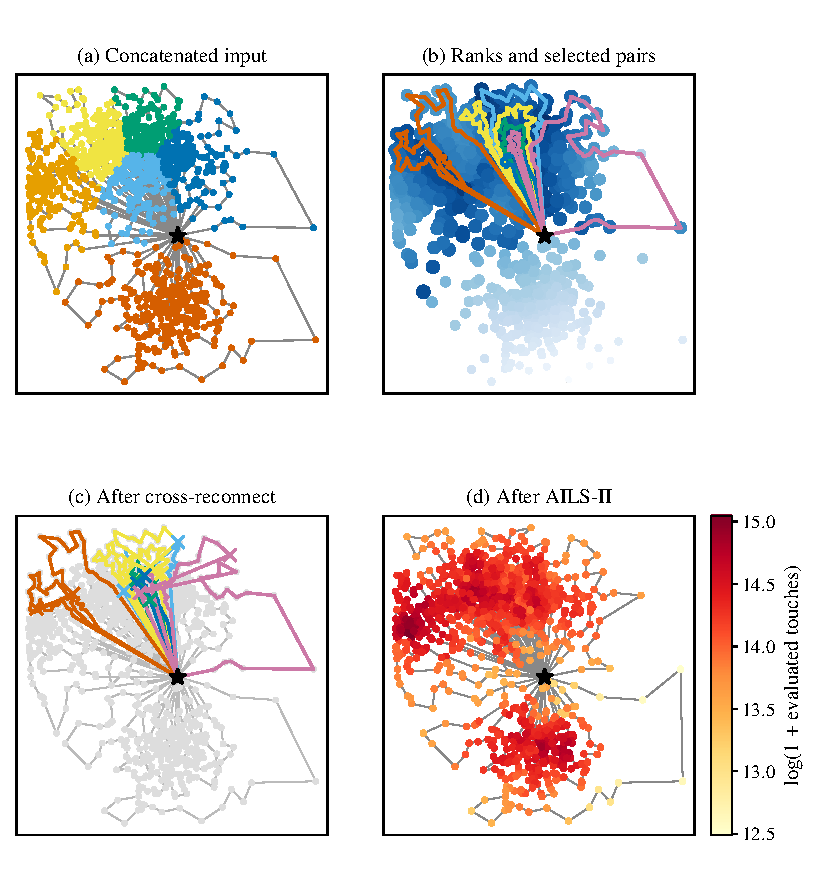
\includegraphics{figures/bgails_mechanism.pdf}
\caption[Illustrative BG-AILS Call on Instance XL-n1281-k29. Colorbar Applies to Panel (d) Only.]{Illustrative \gls{bg-ails} Call on Instance XL-n1281-k29.\\ Colorbar Applies to Panel~(d) Only.}
\label{fig:bgails-mechanism}
\end{figure}
\vspace{-\intextsep}

Table~\ref{tab:hyperparameters} lists the values of the parameters this stage introduces on top of standard AILS-II. Of these, the $\omega$ override and the boundary mask both reach into AILS-II itself. Any other AILS-II hyperparameters governing its own local search and diversification control (the parameters $d_{\min}$, $d_{\max}$, $\gamma$, and $\varphi$ of \citet{maximoHybridAdaptiveIterated2021}) are left at AILS-II's own defaults. Overriding $\omega$ to 10 against AILS-II's own starting value of 30 lowers the solver's internal perturbation degree since \gls{bg-ails} has already displaced customers across subcluster boundaries with its own cross-reconnect chain before AILS-II starts. The subsequent passes are therefore driven to intensify around that disruption rather than to add more of their own. The boundary threshold $\tau$, the small-cluster cap $\sigma$, and the boost $\alpha$ shape the ranks behind both the perturbation weights and the mask. The chain length and the pair-selection rule govern the perturbation step.

The key difference between \gls{bg-ails} and a standard AILS-II improvement pass is therefore this focus on boundary regions, imposed by the perturbation step, by the mask on the first local search, and by the short wall-clock budget \gls{bg-ails} is given. Its budget follows neither the fixed per-customer rate used for subcluster solving (Section~\ref{sec:fra-routing}) nor a plain function of instance size, but a fitted model of the surrounding decompose-route stage's own wall-clock time,
\begin{align}
\text{budget} &= \max\bigl(60\text{s},\ 1.0 \times \widehat{T}_{\mathrm{DR}}\bigr), \label{eq:bg-ails-budget}\\
\widehat{T}_{\mathrm{DR}} &= 0.976 \times n_{\mathrm{waves}}^{-0.180} \times \sum_{\text{waves}} \max(\text{per-cluster budgets in wave}), \label{eq:bg-ails-dr-wall}
\end{align}
refit on 835 pilot \gls{dri} iterations, where waves pack the current iteration's per-subcluster solver budgets (Section~\ref{sec:fra-routing}) into the granted \gls{dri} worker count in partition-submit order. The campaign of Chapter~\ref{chapter:study} runs \gls{bg-ails} asynchronously under this budget: a dedicated worker perturbs and improves the current iteration's solution while the main process decomposes and routes the next one. Section~\ref{sec:fra-pipeline} returns to Equation~\ref{eq:bg-ails-budget} as the quantity that manages the handoff.

Under this comparatively short wall-clock budget, \gls{bg-ails} should outperform an unguided AILS-II pass over the same combined solution, because the unguided pass spends an unknown and likely large share of that budget searching subcluster interiors the decomposition had already solved well. This is tested on all 100 XL instances (Section~\ref{sec:stu-dataset}) at three checkpointed decompose-route solutions each. Three different arms are forked from these checkpoints. The first control arm is a plain AILS-II pass at the solver's own defaults, the second control arm is a blind control that applies one cross-reconnect per subcluster to uniformly drawn route pairs, and the final arm is \gls{bg-ails} in its deployed configuration. Every arm receives the same AILS-II budget. The perturbation of the two perturbing arms is a surplus on top of it, an added median 0.28\% of that budget for \gls{bg-ails} and 0.010\% for the control. The checkpoints are generated under one pinned decomposition configuration, vertex K-Medoids. \gls{haos}, the route pool, and \gls{sc}/\gls{sp} are deactivated, so that the remaining comparison is one improvement stage against another on identical input, not two full runs.

\gls{bg-ails} statistically significantly outperforms both baselines (paired Wilcoxon signed-rank tests, alternative greater, Holm-corrected in a family of two). It improves on the plain AILS-II pass by 0.056~pp of cost improvement over the input solution (Hodges--Lehmann paired difference, 95\% \gls{ci} $[0.049, 0.063]$, Holm-corrected $p = 7.0 \times 10^{-11}$, ahead on 85 of 100 instances) and on the blind control by 0.058~pp (95\% \gls{ci} $[0.052, 0.065]$, Holm-corrected $p = 2.7 \times 10^{-12}$, ahead on 89 of 100). The AILS-II comparison is the practical one and carries the perturbation, the $\omega$ override, and the boundary mask as the package the framework deploys. The control comparison holds $\omega$ and chain length fixed. It measures the placement of the perturbation together with the mask: the blind arm draws its route pairs uniformly and runs AILS-II with no mask. The paired difference between the control and plain AILS-II is consistent with zero (Hodges--Lehmann $-0.004$~pp, 95\% \gls{ci} $[-0.011, 0.002]$), so the gain is not explained by perturbing the concatenated solution at all. Figure~\ref{fig:bgails-comparison} shows the arm means and the paired differences behind those tests.

\begin{figure}[H]
\centering
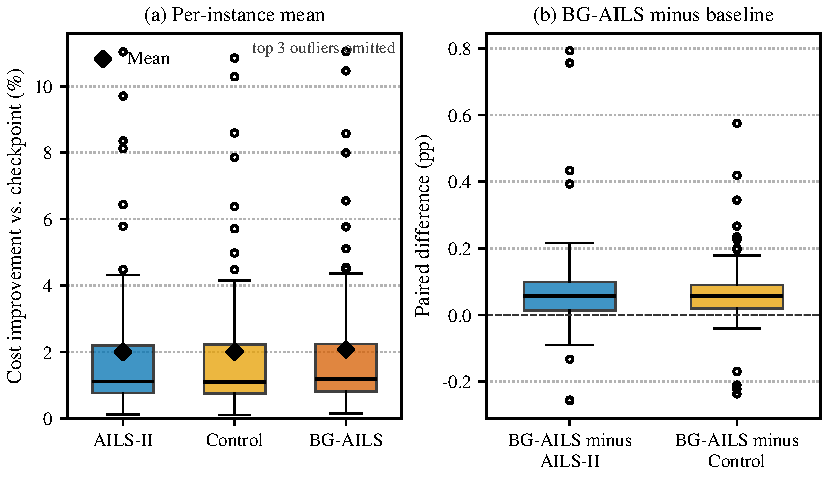
\includegraphics{figures/bgails_comparison.pdf}
\caption[Per-Instance Mean Cost Improvement (a) and Paired BG-AILS Differences (b).]{Per-Instance Mean Cost Improvement (a) and Paired \gls{bg-ails} Differences (b).}
\label{fig:bgails-comparison}
\end{figure}
\vspace{-\intextsep}

However, limiting factors apply. The comparison is only one \gls{dri} iteration, so it says nothing about what these routes are worth once the pool recombines them. It also uses a singular pinned decomposition configuration, under which the clustering and the boundary metric read the same dissimilarity matrix, as they do for three of the eight deployed clustering methods, but not for the five that cluster on raw coordinates or route centroids. And the touch counts in Figure~\ref{fig:bgails-mechanism}(d) come from a separate, identically configured instrumented run rather than from the runs the costs above are measured on.

\gls{bg-ails} finishes the \gls{dri} loop. Its output routes are contributed to the route pool like every other stage's output (Section~\ref{sec:fra-sp}), and the next iteration begins with a fresh \gls{haos} draw over the decomposition and routing operators (Section~\ref{sec:fra-haos}). At fixed intervals, \gls{drispi} recombines the routes accumulated in the pool across many \gls{dri} iterations through set covering or set partitioning, the subject of the next section.

\section[Route Pool and SC/SP Recombination]{\texorpdfstring{Route Pool and \gls{sc}/\gls{sp} Recombination}{Route Pool and SC/SP Recombination}}\label{sec:fra-sp}
Periodically, \gls{drispi} steps back from the current incumbent and recombines every route accumulated so far into one new candidate solution, using set covering or set partitioning (\gls{sc}/\gls{sp}) as the recombination model. Alternating a metaheuristic with an exact set-partitioning solve in this way is an established matheuristic pattern \citep{hybridizing_jourdan_2009}. \citet{cavaliereIntegratedLocalsearchSetpartitioning2022} apply essentially this pairing to large-scale \gls{cvrp} instances directly, by alternating LKH-3 local search with a restricted set-partitioning solve. Doing so only pays off if a shared memory of routes exists for it to recombine. So this section first describes that memory, the route pool, before turning to the \gls{sp} and \gls{sc} models themselves and the hyperparameter that decides between them.

The route pool stores one entry per distinct customer set $C_r \subseteq C$, where $C$ is the customer set of the instance (Section~\ref{sec:lit-problem}), keyed by the frozen customer set rather than by the ordered sequence of customers a route visits them in. Two routes serving the same customers in a different order, or at a different cost, are treated as the same column, and the cheaper of the two overwrites the other. This column-oriented memory, populated online during the \gls{dri} loop and periodically recombined through a partitioning model, follows the adaptive-memory principle of \citet{rochatProbabilisticDiversificationIntensification1995}, who introduce the route pool and its set-partitioning recombination for vehicle routing.

Routes are fed to the pool following a contribute-before-adopt rule, which adds a candidate solution to the pool before the pipeline decides whether to adopt it as the new incumbent, so a losing candidate still leaves its routes behind for later reuse. The \gls{dri} loop contributes to the pool twice per iteration, once from its decompose-route stage (Section~\ref{sec:fra-routing}) and once from the following improvement stage (\gls{bg-ails} (Section~\ref{sec:fra-bg-ails})). The \gls{sc}/\gls{sp} step covered in this section feeds the pool only indirectly. Solving \gls{sc} or \gls{sp} selects among the customer sets already in the pool and creates no new ones, so its own output adds nothing. Every contributed route carries a tag recording the full \gls{haos} selection that produced it, that is, $k$, the demand weight, the paradigm, the method, and the solver, with a separate flag marking routes from the post-\gls{sc}/\gls{sp} improvement pass. Whenever a candidate is adopted as the new incumbent, its routes, already in the pool by the rule above, are marked elite. Elite routes are exempt from ever being evicted from the pool to ensure the incumbent is never lost.

Every \gls{sc}/\gls{sp} solve also updates two running scores on each pool entry, A quality and a diversity score. The quality score represents a column's usefulness for the solver during the \gls{sc}/\gls{sp} solve. Therefore, an entry never touched by a solve carries no quality score yet. The diversity score is the mean Jaccard distance \citep{jaccardDistributionFloreAlpine1901} between a route's customer set and every other pool entry's customer set,
\begin{equation}
\bar{J}(r) = \frac{1}{|R| - 1} \sum_{r' \in R \setminus \{r\}} \frac{|C_r \triangle C_{r'}|}{|C_r \cup C_{r'}|},
\label{eq:route-diversity}
\end{equation}
where $R$ is the pool at the time of the update, recomputed for every entry whenever any solve happens. New quality or diversity scores are appended to a three-value window, from which final scores are read as the mean of their respective window. This ensures that single unusually high or low values do not dominate a route's standing.

These scores are a route's critical metrics when it comes to eviction from the pool. Eviction is necessary, because the route pool has a maximum size (10,000 columns by default) to keep the computational complexity of the \gls{sc}/\gls{sp} solve from blowing up. Therefore, an eviction policy is established that ranks the non-elite entries on both quality and diversity and combines their ranks into one fitness value. Among the entries that have been scored at least once, ascending order by mean quality score gives rank one to the weakest route and the highest rank to the strongest. Independently, ascending order by mean diversity score gives rank one to the most redundant route and the highest rank to the most unique. Using $\rho_q(r)$ and $\rho_d(r)$ for these two ranks, fitness is $\Phi(r) = \rho_q(r) + w_d \cdot \rho_d(r)$, with the diversity weight $w_d$ (0.5 by default) controlling how much redundancy counts against a route relative to raw quality. The entries with the lowest $\Phi(r)$ are evicted first. Because both terms grow towards the same end of their respective orderings, a route that the \gls{sc}/\gls{sp} solve relies on heavily, but that is also nearly identical to several other pool entries, can rank as a stronger eviction candidate than a weak but singular one, because redundancy drives the diversity term up regardless of quality. The eviction policy only triggers once the pool exceeds its maximum size and then only removes the overflow amount. Unscored entries are evicted only if the overflow cannot be covered by scored, non-elite entries alone.

The recombination model itself treats the pool as a column set. Let $R$ be the set of routes currently in the pool, $c_r$ the cost of route $r \in R$, that is, the Euclidean depot-customers-depot round trip over the travel costs of Section~\ref{sec:lit-problem}, and $x_r \in \{0, 1\}$ a decision variable selecting route $r$. Set partitioning, in the formulation \citet{balinskiIntegerProgramDelivery1964} introduce for exactly this delivery-routing setting, reads
\begin{align}
\text{min} \quad & \sum_{\mathclap{r \in R}} c_r x_r \label{eq:sp-obj}\\
\text{s.t.} \quad & \sum_{\mathclap{r \in R:\, i \in C_r}} x_r = 1, && \forall i \in C \label{eq:sp-partition}\\
& x_r \in \{0, 1\}, && \forall r \in R. \label{eq:sp-binary}
\end{align}
Solving Equations~\ref{eq:sp-obj}--\ref{eq:sp-binary} recombines route fragments that have never been jointly considered, for example because they may have entered the pool from different subclusters, different \gls{haos} draws, or different iterations, into one coherent solution that still covers every customer exactly once. This is the sense in which \gls{sp} looks across the boundaries any individual \gls{dri} iteration's decomposition imposes, something no individual subcluster solve or \gls{bg-ails} perturbation can do on its own.

\gls{drispi} builds this model once using Gurobi\footnote{\url{https://www.gurobi.com}} and solves it twice. It first relaxes Equation~\ref{eq:sp-binary} to the continuous $x_r \in [0, 1]$ and solves the resulting linear program. This \gls{lp} relaxation allows the solver to assign fractional weights rather than the binary ones to each route, making it significantly easier and faster to solve. The resulting fractional weights are then utilized as the quality scores fed back into the route pool above, so every \gls{sc}/\gls{sp} solve doubles as a scoring pass over the pool regardless of what it ultimately selects. This follows the same spirit in which column-generation approaches read pricing information out of \gls{lp} duals \citep{lubbeckeSelectedTopicsColumn2005}. For the second solve, the variables are then switched to binary, warm-started from the \gls{lp} solution, and re-optimized as a mixed-integer program under a wall-clock time limit and a relative optimality gap (720 seconds and 0.025\% by default). A wallclock time limit is required to cut off the search with a good, if not provably optimal, solution.

The equality constraint of Equation~\ref{eq:sp-partition} is only a meaningful choice if the pool offers more than one real alternative for most customers. A pool still dominated by a single incumbent partition would just reproduce it again and again under \gls{sp}. \gls{drispi} therefore checks, before the \gls{sc}/\gls{sp} is triggered, whether every customer in the instance is covered by at least a fixed minimum number of pool routes (five by default). Only when that holds does \gls{sp} run. Otherwise \gls{drispi} falls back to the less constrained set covering (\gls{sc}), the inequality-constrained relaxation of the same formulation \citep{garfinkelSetPartitioningProblemSetCovering1969}, whose formal problem statement and \gls{lp} relaxation are given in Appendix~\ref{app:set-covering}. \gls{sc} only requires every customer to be covered at least once rather than exactly once. Under the cover inequality a thin pool takes up a single alternative route together with the incumbent routes it overlaps, whereas the equality admits that route only once other columns fill exactly the customers it displaces. Both, \gls{sp} and \gls{sc} are safe and never blocked by infeasibility, only by a pool that has not yet accumulated enough alternatives. \gls{sc} exists to give the step something useful and always solvable to run on every scheduled trigger, warmup aside, no matter how much the pool has matured. The price of \gls{sc}'s additional permissiveness is that selected routes can overlap on a customer, meaning a customer can be visited by more than a single route and therefore more than exactly once. Since this would violate the problem statement formulated in Section~\ref{chapter:problem}, a savings-based deduplication heuristic then removes each duplicated customer from every selected route except the one where removing it would save the least cost, restoring a feasible partition.

A solved partitioning problem will pair routes into a new candidate solution which haven't been evaluated together before. And while search heuristics have been employed in identifying the routes used, the resulting new set of routes has not been polished by evaluating for example inter-route moves amongst each other. To do just that the \gls{sc}/\gls{sp} step is combined with a post-\gls{sc}/\gls{sp} improvement pass (Section~\ref{sec:fra-improve}) to improve the partitioning result even further if possible.

\section{Post-Recombination Improvement}\label{sec:fra-improve}
Once \gls{sc}/\gls{sp} (Section~\ref{sec:fra-sp}) recombines the route pool into one partition, \gls{drispi} runs one further pass over it using AILS-II as solver, seeded only with that partition as an initial solution. Unlike in \gls{bg-ails} (Section~\ref{sec:fra-bg-ails}), this step focuses less on perturbation but rather refinement by local search. This post-recombination improvement pass also allows the solver to touch all routes instead of guiding moves towards certain neighborhoods. The pass runs under its own wall-clock budget (360 seconds by default) on the same core reservation as the \gls{sc}/\gls{sp} solve that precedes it. Section~\ref{sec:fra-pipeline} elaborates how exactly a parallel architecture of \gls{drispi} looks.

The refined routes feed back into the route pool exactly like every other stage's output (see Section~\ref{sec:fra-sp}). A route whose customer set matches one \gls{sc}/\gls{sp} already selected keeps that route's existing tag, while a route created by moving customers between routes in this stage is added as new, and tagged as an improvement route rather than credited to an existing \gls{haos} selection.

This is also where the deferred rewards of \gls{haos} are distributed (Section~\ref{sec:fra-haos}). The pass's outcome, a new best, an improvement over the previous iteration without beating the incumbent, or neither, is scored through the deferred branch of \gls{haos}'s reward function and credited not to the current iteration's own draw but to every distinct \gls{haos} tag the routes \gls{sc}/\gls{sp} selected already carried. That is, to whichever earlier decompose-route or \gls{bg-ails} draws produced those specific routes, regardless of how many iterations ago that was. Improvement-route tags are excluded from this credit, since this stage created them without any \gls{haos} draw of their own to reward.

\section{Parallelized Pipeline Orchestration}\label{sec:fra-pipeline}
The preceding sections describe \gls{haos}, decomposition, routing, \gls{bg-ails}, the route pool and \gls{sc}/\gls{sp}, and the post-\gls{sc}/\gls{sp} improvement pass as if they were executed sequentially, like Figure~\ref{fig:dri-overview} shows. And while \gls{drispi}'s implementation allows for sequential execution, it also offers a more potent, highly parallelized mode as well. For that it splits eight cores into three disjoint groups and distributes six for the main loop and the \gls{dri} routing pool of Section~\ref{sec:fra-routing}, one for the \gls{bg-ails} worker of Section~\ref{sec:fra-bg-ails}, and one for the \gls{sc}/\gls{sp} and post-\gls{sc}/\gls{sp} improvement worker of Sections~\ref{sec:fra-sp} and~\ref{sec:fra-improve}. A main orchestration process shares the six \gls{dri} cores rather than occupying a ninth.

Figure~\ref{fig:pipeline-swimlane} shows what this asynchronous, parallelized mode looks like across two consecutive iterations. After decompose-route of iteration~$i$ the loop waits for job~$i{-}1$ and drains it~\mk{1}, then launches job~$i$ on the new solution~\mk{2}. After decompose-route of iteration~$i{+}1$ the same pair of steps waits for job~$i$, drains it, and launches job~$i{+}1$. A finished \gls{sc}/\gls{sp} job is drained without blocking~\mk{3} at the start of the following iteration.

\begin{figure}[tbp]
\centering
\resizebox{\linewidth}{!}{% ---------------------------------------------------------------------------
% DRISPI parallelized pipeline, iterations i and i+1 (schematic).
% Requires: arrows.meta, patterns, decorations.pathreplacing, calc
% Block lengths are illustrative; the order of events follows the main loop.
% ---------------------------------------------------------------------------
\begin{tikzpicture}[
  font=\small\normalfont,
  >={Latex[length=1.8mm]},
  blk/.style={draw, thick, minimum height=0.8cm, inner sep=1pt, anchor=west,
              align=center, font=\footnotesize},
  dr/.style={blk, fill=blue!12},
  hs/.style={blk, fill=blue!30!black!80, text=white, font=\scriptsize\normalfont\bfseries},
  bg/.style={blk, fill=orange!18},
  wait/.style={draw, thick, pattern=north east lines, pattern color=black!45,
               minimum height=0.8cm, inner sep=0pt, anchor=west},
  launch/.style={->, thick},
  drain/.style={->, thick, dashed},
  num/.style={circle, draw, thick, fill=white, inner sep=0.6pt,
              font=\scriptsize\bfseries, minimum size=3.6mm},
  lbl/.style={font=\scriptsize},
]
\def\yD{0}\def\yB{-1.4}\def\yS{-2.8}
\def\h{0.4}
\def\pblk#1#2#3#4#5{\node[#1, minimum width=#4cm-#3cm] at (#3,#2) {#5};}

% ---- lanes -----------------------------------------------------------------
\foreach \y/\n/\c in {\yD/DRI-Loop/6 cores, \yB/BG-AILS/1 core, \yS/SP/1 core}{
  \node[anchor=east, align=right] at (-0.35,\y) {\n\\[-1pt]{\scriptsize (\c)}};
  \draw[black!20] (-0.2,\y) -- (11.6,\y);
}

% ---- iteration brackets ------------------------------------------------------
\draw[decorate, decoration={brace, amplitude=5pt}, thick]
  (0,\yD+\h+0.12) -- node[above=5pt] {iteration $i$} (5.7,\yD+\h+0.12);
\draw[decorate, decoration={brace, amplitude=5pt}, thick]
  (5.8,\yD+\h+0.12) -- node[above=5pt] {iteration $i{+}1$} (11.0,\yD+\h+0.12);

% ---- DRI-Loop --------------------------------------------------------------
\pblk{hs}{\yD}{0}{0.35}{H}
\pblk{dr}{\yD}{0.35}{4.8}{decompose\,+\,route $i$}
\node[wait, minimum width=0.6cm] at (4.8,\yD) {};
\pblk{hs}{\yD}{6.2}{6.55}{H}
\pblk{dr}{\yD}{6.55}{10.8}{decompose\,+\,route $i{+}1$}

% ---- bg --------------------------------------------------------------------
% BG-AILS i-1 was launched at the end of iteration i-1 (open left edge)
\fill[orange!18] (-0.2,\yB-\h) rectangle (5.4,\yB+\h);
\draw[thick] (-0.2,\yB-\h) -- (5.4,\yB-\h) -- (5.4,\yB+\h) -- (-0.2,\yB+\h);
\node[font=\footnotesize] at (2.7,\yB) {BG-AILS $i{-}1$};
\pblk{bg}{\yB}{5.6}{9.9}{BG-AILS $i$}
\node[lbl, text=black!60] at (10.35,\yB) {idle};
\fill[orange!18] (11.0,\yB-\h) rectangle (11.6,\yB+\h);
\draw[thick] (11.6,\yB-\h) -- (11.0,\yB-\h) -- (11.0,\yB+\h) -- (11.6,\yB+\h);
\node[font=\footnotesize] at (11.3,\yB) {$i{+}1$};

% ---- sp --------------------------------------------------------------------
% SC/SP job dispatched at an earlier trigger (open left edge)
\fill[black!8] (-0.2,\yS-\h) rectangle (3.4,\yS+\h);
\draw[thick] (-0.2,\yS-\h) -- (3.4,\yS-\h) -- (3.4,\yS+\h) -- (-0.2,\yS+\h);
\node[font=\footnotesize] at (1.6,\yS) {SC/SP\,+\,AILS-II};
\node[lbl, text=black!60, anchor=west] at (3.55,\yS) {done};
\node[lbl, text=black!60, anchor=west] at (6.55,\yS) {idle until the next trigger};

% ---- handoffs ----------------------------------------------------------------
% end of iteration i: wait for BG i-1, drain it, launch BG i
\draw[drain]  (5.4,\yB+\h) -- (5.4,\yD-\h);
\draw[launch] (5.6,\yD-\h) -- (5.6,\yB+\h);
\node[num] at (5.12,-0.7) {1};
\node[num] at (5.83,-0.7) {2};
% start of iteration i+1: drain the finished SC/SP job (non-blocking)
\draw[white, line width=3.5pt] (6.12,\yB-\h) -- (6.12,\yB+\h);
\fill (6.12,\yS) circle (1.5pt); \draw[drain] (6.12,\yS) -- (6.12,\yD-\h);
\node[num] at (6.4,-2.1) {3};
% end of iteration i+1: BG i already finished, no wait
\draw[drain]  (10.8,\yB+\h) -- (10.8,\yD-\h);
\draw[launch] (11.0,\yD-\h) -- (11.0,\yB+\h);
\node[num] at (10.52,-0.7) {1};
\node[num] at (11.28,-0.7) {2};

% ---- one-iteration lag -------------------------------------------------------
\draw[decorate, decoration={brace, amplitude=4pt, mirror}, thick]
  (6.55,\yD-\h-0.1) -- node[lbl, below=4pt, fill=white, inner sep=1pt] {runs alongside BG-AILS $i$} (9.9,\yD-\h-0.1);

% ---- legend ----------------------------------------------------------------
\begin{scope}[shift={(0,-3.85)}, every node/.style={lbl, anchor=west}]
  \node[num, anchor=center] at (0.15,0)     {1}; \node at (0.35,0)     {wait for the previous BG-AILS job and drain it};
  \node[num, anchor=center] at (0.15,-0.45) {2}; \node at (0.35,-0.45) {launch BG-AILS on the new solution};
  \node[num, anchor=center] at (0.15,-0.9)  {3}; \node at (0.35,-0.9)  {drain a finished SC/SP job (non-blocking)};
  \node[hs, anchor=center, minimum height=3.6mm, minimum width=3.6mm] at (7.0,0) {H};
  \node at (7.2,0) {HAOS draw};
  \node[wait, anchor=center, minimum width=3.6mm, minimum height=3.6mm] at (7.0,-0.45) {};
  \node at (7.2,-0.45) {main loop blocked};
\end{scope}
\end{tikzpicture}
}
\caption[Two Consecutive DRISPI Iterations in One 8-Core Container (6 for DRI, 1 for BG-AILS, and 1 for SP). Block Lengths Are Illustrative.]{Two Consecutive \gls{drispi} Iterations in One 8-Core Container 
(6 for \gls{dri}, 1 for \gls{bg-ails}, and 1 for \gls{sp}). Block Lengths Are Illustrative.}
\label{fig:pipeline-swimlane}
\end{figure}

Equation~\ref{eq:bg-ails-budget} sizes the \gls{bg-ails} budget to the decompose-route stage it overlaps with, which is what keeps the wait at~\mk{1} short. A budget much shorter than the next decompose-route pass would leave the \gls{bg-ails} core idle before the handoff. A budget much longer would leave the \gls{dri} cores blocked on a job that already had the next iteration's input ready. In Figure~\ref{fig:pipeline-swimlane} the wait after decompose-route of iteration~$i{+}1$ vanishes because job~$i$ finished during that pass.

The \gls{sc}/\gls{sp} worker uses a skip policy rather than a blocking handoff. The campaign checks the trigger only at iteration boundaries, so a job starts at the first boundary after the x-minute mark (20 by default), not exactly at it. \gls{drispi} then dispatches a snapshot of the route pool and the incumbent only if the worker is idle. If it is busy, the trigger is skipped rather than queued. The worker owns both the \gls{sc}/\gls{sp} solve and the post-\gls{sc}/\gls{sp} improvement pass of Section~\ref{sec:fra-improve}, running them one after another on the same core. Those two default ceilings, 720~s and 360~s, sum to 18 minutes and therefore leave two minutes of slack under the default 20-minute interval. A skip is therefore only necessary if enqueue and overhead consume that slack.

Algorithm~\ref{alg:pipeline} shows the complete and deployed \gls{drispi} loop. After decompose-route the loop waits for the previous \gls{bg-ails} job~\mk{1}, drains it through Absorb, and launches the next job on $(S_{\mathrm{DR}}, \kappa, \lambda_q)$~\mk{2}, keeping $\theta$ only for later credit. A finished \gls{sc}/\gls{sp} job is absorbed without blocking~\mk{3} at the start of the next iteration. A synchronous mode that runs both stages inline is implemented as a code option and recovers the sequential picture of Figure~\ref{fig:dri-overview}.

\begin{algorithm}[tbp]
\caption{\gls{drispi} Main Loop as Deployed (Async. \gls{bg-ails} and \gls{sp})}\label{alg:drispi}\label{alg:pipeline}
\KwIn{instance; time limit $\Gamma$}
\KwInit{$R \gets \emptyset$; $S^\star$ undefined; $i \gets 0$}
\BlankLine
\While{elapsed time $< \Gamma$}{
  \If{the \gls{sc}/\gls{sp} job has finished}{
    \Absorb{$S_{\mathrm{\gls{sp}}}, \Theta_{\mathrm{\gls{sp}}}$, deferred} \tcp*[r]{$\Theta_{\mathrm{\gls{sp}}}$: tags of selected routes}
  }
  $(\theta, \text{config}) \gets \Draw{$S^\star$}$ \tcp*[r]{Algorithm~\ref{alg:haos}}
  decompose into $k$ subclusters under config \tcp*[r]{Section~\ref{sec:fra-decomposition}}
  \ParFor{each subcluster}{route it with the drawn solver \tcp*[r]{Section~\ref{sec:fra-routing}}}
  $S_{\mathrm{DR}} \gets$ concatenated subcluster routes; \Absorb{$S_{\mathrm{DR}}, \{\theta\}$, immediate}\;
  \If{a \gls{bg-ails} job is in flight}{
    wait for its result $(S_{\mathrm{BG}}, \theta')$; \Absorb{$S_{\mathrm{BG}}, \{\theta'\}$, immediate}\;
  }
  dispatch \gls{bg-ails} on $(S_{\mathrm{DR}}, \kappa, \lambda_q)$ \tcp*[r]{Algorithm~\ref{alg:bgails}; $\theta$ for credit}
  \If{\gls{sc}/\gls{sp} is due \KwAnd the sp worker is idle}{
    dispatch \SPJob{$R, S^\star$} to the sp worker\;
  }
  \Decay{}; $i \gets i + 1$\;
}
\Return $S^\star$\;
\BlankLine
\Fn{\Absorb{$S, \Theta$, channel}}{
  $r \gets$ reward of $S$ in this channel (Table~\ref{tab:haos-rewards})\;
  add the routes of $S$ to $R$; \lIf{$c(S) < c(S^\star)$}{$S^\star \gets S$}
  \lForEach{$\theta \in \Theta$}{\Credit{$\theta, r$}}
}
\BlankLine
\Fn{\SPJob{$R, S^\star$}}{
  \leIf{min.\ coverage of $R \geq 5$}{$S \gets \mathrm{\gls{sp}}(R)$}{$S \gets \mathrm{dedup}(\mathrm{\gls{sc}}(R))$}
  \Return $\solver(S)$ under the improvement budget \tcp*[r]{Section~\ref{sec:fra-improve}}
}
\end{algorithm}

This Algorithm~\ref{alg:pipeline} is the loop the following Chapter~\ref{chapter:study} evaluates. It is run, unchanged, on all 100 XL instances under a two-hour budget, and the resulting costs are compared with the monolithic solvers benchmarked on that set.